\section[Introdução]{Introdução}

O projeto foi concebido a partir de uma ``dor'' identificada pelas \textit{stakeholders} Eliza Pasquali Lunardi e Letícia Fossá Rosa, fundadoras do Estudify e vencedoras do Startup Garagem. Embora já possuíssem uma plataforma web funcional de preparação para o ENEM e vestibulares com usuários pagantes, as clientes enfrentavam limitações na experiência oferecida aos estudantes e dificuldades recorrentes na gestão de conteúdo, identificando a necessidade de evoluir o produto para uma aplicação \textit{mobile} nativa, mais engajadora e alinhada ao comportamento do público jovem.

O projeto teve como objetivo tornar o estudo para o ENEM e vestibulares mais leve e eficiente, por meio de uma experiência gamificada inspirada no Duolingo. Foi proposto um aplicativo \textit{mobile} em que o estudante aprende resolvendo questões organizadas por disciplina e tópico, com \textit{feedback} instantâneo via gabarito comentado, complementado por simulados completos no formato ENEM, cronograma personalizado de estudos e um sistema de gamificação com moedas, \textit{streaks} diários e acompanhamento de progresso. O projeto também contemplou um painel administrativo web, destinado às clientes, para importação em lote de questões e acompanhamento dos usuários.

A execução do projeto ocorreu no primeiro semestre de 2026, entre os dias 02 de março e 29 de junho de 2026, compreendendo diversas etapas realizadas pelos estudantes do bacharelado em Engenharia de Software no âmbito da \ac{ages}, sob a orientação do professor Marcelo H. Yamaguti. A foto do time responsável pelo projeto pode ser vista na Figura~\ref{fig:estudify-time}.

\begin{figure}[H]
    \centering
    \small
    \caption{Time do projeto Estudify}
    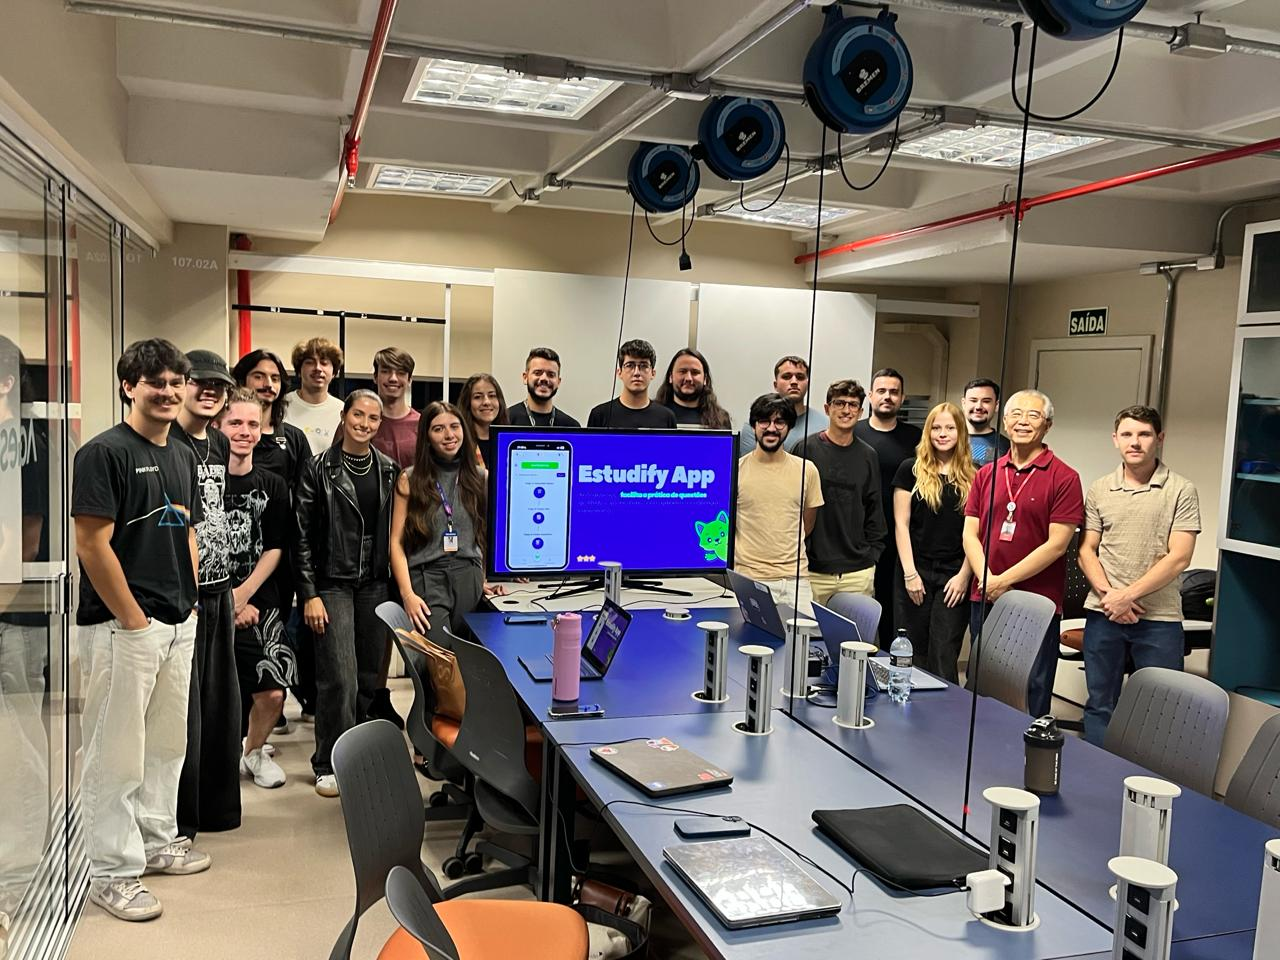
\includegraphics[width=0.9\linewidth]{conteudo/5 - ages IV/images/fig11-time-estudify.png}

    Fonte: Wiki do projeto
    \label{fig:estudify-time}
\end{figure}
